\chapter{Mathe - Klasse 1}
\section{Übungen 1}
Rechne aus: \\ \\
\begin{tabular}{p{1cm}p{1cm}p{1cm}p{1cm}p{1cm}}
  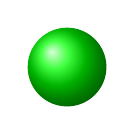
\begin{tikzpicture}
    \shade[ball color=green] (9,0.5) circle (0.5cm); 
  \end{tikzpicture} &
  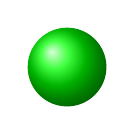
\begin{tikzpicture}
    \shade[ball color=green] (9,0.5) circle (0.5cm);
  \end{tikzpicture} &
  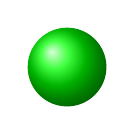
\begin{tikzpicture}
    \shade[ball color=green] (9,0.5) circle (0.5cm); 
  \end{tikzpicture}
\end{tabular}

\begin{tabular}{p{1cm}p{1cm}p{1cm}p{1cm}p{1cm}}
  &
  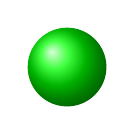
\begin{tikzpicture}
    \shade[ball color=green] (9,0.5) circle (0.5cm); 
  \end{tikzpicture}
\end{tabular}

\vspace{1.5cm}

\begin{tabular}{p{1cm}p{1cm}p{1cm}p{1cm}p{1cm}}
  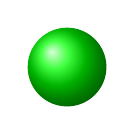
\begin{tikzpicture}
    \shade[ball color=green] (9,0.5) circle (0.5cm); 
  \end{tikzpicture} &
  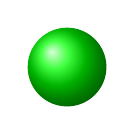
\begin{tikzpicture}
    \shade[ball color=green] (9,0.5) circle (0.5cm);
  \end{tikzpicture} &
  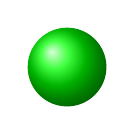
\begin{tikzpicture}
    \shade[ball color=green] (9,0.5) circle (0.5cm); 
  \end{tikzpicture}
\end{tabular}


\vspace{1.5cm}
\hspace{0.75cm}
\begin{tabular}{p{1.0cm}p{1.0cm}}
  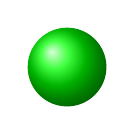
\begin{tikzpicture}
    \shade[ball color=green] (9,0.5) circle (0.5cm);
  \end{tikzpicture} &
  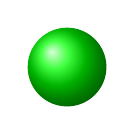
\begin{tikzpicture}
    \shade[ball color=green] (9,0.5) circle (0.5cm); 
  \end{tikzpicture}
\end{tabular}


\vspace{1.5cm}
\hspace{0.75cm}
\begin{tabular}{p{1.0cm}p{1.0cm}}
  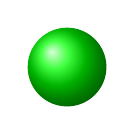
\begin{tikzpicture}
    \shade[ball color=green] (9,0.5) circle (0.5cm);
  \end{tikzpicture} &
  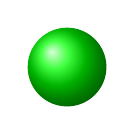
\begin{tikzpicture}
    \shade[ball color=green] (9,0.5) circle (0.5cm); 
  \end{tikzpicture}
\end{tabular}


\vspace{1.5cm}
\hspace{1.50cm}
\begin{tabular}{p{1.0cm}}
  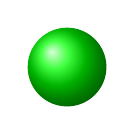
\begin{tikzpicture}
    \shade[ball color=green] (9,0.5) circle (0.5cm); 
  \end{tikzpicture}
\end{tabular}
